\section{Comparison}
\label{sec:comparison}
\textcolor{red}{to other implementations, to biology\\}
% original paper
The authors of \cite{SNN}  present an unsupervised approach to train a \ac{SNN} model.
However, there are other approaches to train \acp{SNN}, as well as opions with regard to the biological plausibility of the methods used.


% STDP-like paper
The \ac{SNN} model from \cite{STDP_like} determines its output by 
choosing the class of the first neuron pool to reach the descision threshold with its accumulated sensory evidence.
The authors claim that the original method of using a majority vote of single threshold-based neuron acticity is less biologically plausible.

Not only the \cite{STDP_like} model but also the \cite{SNN} model use inhibition.

The authors of \cite{STDP_like} point out that the classifier neuron will not recognize atypical digits (i.e. their stimulus).
Therefore, the ability to generalize on new datasets depends on the inputs' similiarity to the learned patterns.


% DIET-SNN paper

% Captial L to avoid strange behaviour since figure is close to page break
\begin{wrapfigure}{L}{0.25\textwidth}
    \centering
    \vspace{-20pt}
    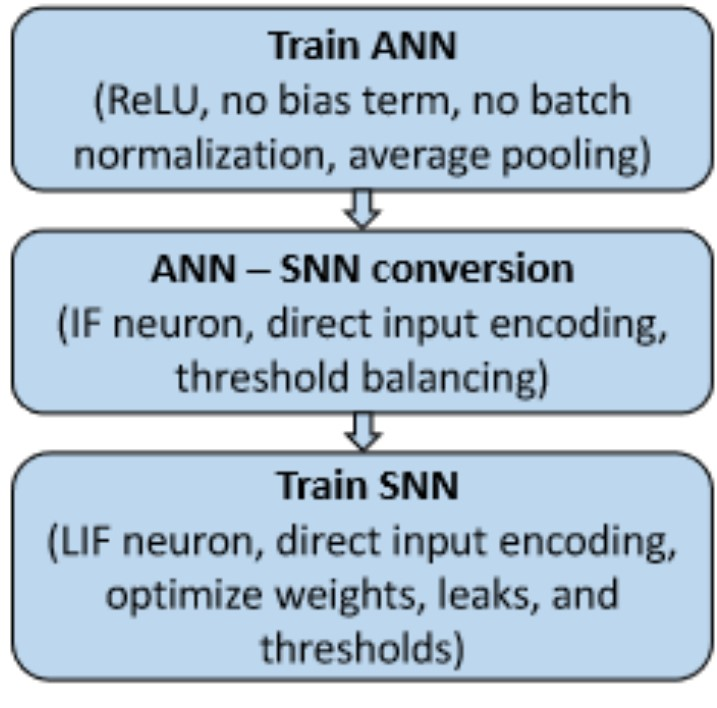
\includegraphics[width=0.25\textwidth]{pictures/DIET_SNN_pipeline.jpg}
    \caption{\acs{DIET}-\ac{SNN} training pipeline from \cite{DIET_SNN}}
    \label{fig:training_pipeline_DIET_SNN}
\end{wrapfigure}

The \ac{DIET}-\ac{SNN} model from \cite{DIET_SNN} is an entriely different approach to those discussed before.
As depicted in \autoref{fig:training_pipeline_DIET_SNN}, an \ac{ANN} is trained and thereafter converted into a \ac{SNN}.
The initialized parameters speed up the subsequent training wit spike-based backpropagation.
Instead of using a Poisson generator (rate-coding: converting analog values to spike-train),the image pixels are directly applied as input.
The first convolutional layer is trained to encode them as spikes.

\textcolor{red}{
This alternative approach uses supervised learning of \acs{DIET}-\ac{SNN} proposed by \cite{DIET_SNN}.
The \ac{DIET}-\ac{SNN} model's first layer is trained to encode the input as spikes.
The pixel intensities of an image are directly applied to the first convolutional layer's \ac{LIF} neurons.
The neurons accumulate the weighted pixel and generate ouput spikes.
This encoding is learned beforehand using gradient-descent.
%
\begin{equation}
    \centering
    \label{eq:DIET-SNN-membrane-potential}
    u_i^t = \lambda_i u_i^{t-1} + \sum_{j}^{}w_{ij}o_j^t-v_{i}o_i^{t-1}
\end{equation}
%
The membrane potential $u_i^t$ of a postsynaptic neuron $i$ at timestep $t$ 
is calculted using \autoref{eq:DIET-SNN-membrane-potential} from \cite{DIET_SNN}. 
$\lambda_i \in [0,1]$ is the leak factor of the membrane potential, 
$w_{ij}$ the weight of the synapse between neuron $i$ and $j$, 
$o_j^t$ the output spike of neuron $j$ at timestep $t$ and 
$v_i$ the threshold of neuron $i$.
The first term calculates the leakage of the neuron,
the second term the accumulated input of the presynaptic neurons and
the third term enables a soft reset (reducing by threshold $v_i$ instead of reset to zero) of the membrane potential after a spike was generated.
}